\chapter{Implementation}
\label{chap:impl}

We implemented a super-harness that takes an existing benchmark harness as an input and executes its benchmarks in the asynchronous duet style.

% Running in docker and reasons for it
To keep a configuration portable and the dependencies minimal we have decided to use the container technology, namely Docker~\cite{merkel2014docker} or Podman~\footnote{\url{https://podman.io/}, July 2022}.
Tool is named \lstinline{duetbench} and it is part of open sourced~\footnote{Apache Licence 2.0} python package \lstinline{duet}~\footnote{\url{https://github.com/TomasDrozdik/asynchronous-duet}, July 2022} that also implements other complementary tools described in~\cref{sec:result_parsing}.
Source code is available as an attachment to this thesis~\xxx{ref} and it has documentation in form of GitHub wiki~\cite{wiki}.

We want to compare asynchronous duet with~\citet{bulej2020duet}, hence our super-harness supports synchronized duet and sequential method in a containerized environment.

\section{Architecture}

\Cref{fig:duetbench_sequence} depicts architecture of \lstinline{duetbench} script.
\lstinline{duetbench} is a process on the host machine that spawns subprocesses that run containers --- one for each version A/B.
Since initialization of a container might take longer \lstinline{duetbench} waits for both containers to start and then uses \lstinline{docker exec}~\footnote{\url{https://docs.docker.com/engine/reference/commandline/exec/}} to run the command that executes the benchmark harness loop from~\cref{alg:harness}.
Once both benchmarks finish, copy the raw result of those benchmarks from their respective containers and store them in a predefined directory structure that preserves super-harness metadata and raw results~\cite{wiki}.
Afterward, stop and clean up both containers.
We refer to this process as a \emph{run} and it is analogous to a \emph{trial} from~\citet{laaber2019software} and~\citet{abedi2017conducting} for sequential runs.
For duet methods, one \emph{run} executes 2 benchmarks in parallel.

\begin{figure}
    \centering
    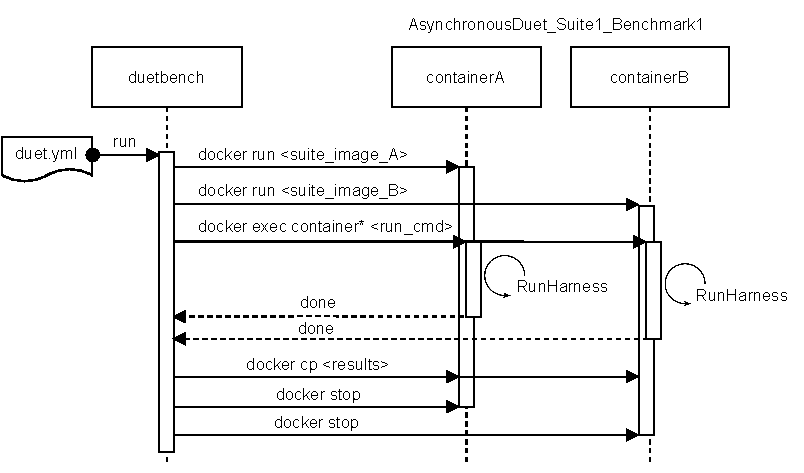
\includegraphics[width=\linewidth]{./figures/duetbench-sequence.drawio.pdf}
    \caption{
        UML sequence diagram of how \lstinline{duetbench} executes a single A/B asynchronous duet benchmark.
        All the parameters in angled brackets are specified in the configuration file \lstinline{duet.yml} described in~\cref{sec:configuration}.
        Note that the docker commands are simplified for brevity.
    }
    \label{fig:duetbench_sequence}
\end{figure}

If there are more benchmarks to execute pick the next one (according to a particular scheduling strategy, see~\cref{sec:scheduling}) and do the same process.
In the case of the sequential method, the process is very much the same just omit the second container entirely and run them separately.

\subsection{Synchronized duet in containerized environment}
\label{sec:sync_duet_impl}

\citet{bulej2020duet} uses a \mbox{shared-memory} barrier to synchronize benchmark iterations.
We ported this solution into the containers to mimic the original behavior.

The barrier uses the pthread API that is not available on all systems such as macOS.
Therefore, \lstinline{duetbench} starts a third container to initialize, and later clean up the barrier, hence bypassing the missing functionality on the host system.

Docker environments are separated by design.
To facilitate this feature \lstinline{duetbench} mounts host directory \lstinline{-v /dev/shm:/dev/shm} and shares \mbox{inter-process} communication namespace \lstinline{--ipc host}~\footnote{\lstinline{docker run} reference \url{https://docs.docker.com/engine/reference/run/}}.

\subsection{Run Scheduling}
\label{sec:scheduling}

\lstinline{duetbench} supports two options for \emph{run scheduling}:
\begin{description}
    \item[Sequential] where benchmarks are run in order of definition from a configuration file.
    \item[Randomized Interleaving Trials] where it randomly interleaves the runs from a configuration file.
        Hence, it can mix different types of measurement methods and benchmarks.
        With multiple repetitions of a given measurement method, it is essentially RMIT\cite{abedi2017conducting}.
\end{description}

\section{Configuration}
\label{sec:configuration}

\Cref{lst:config} shows section of \lstinline{duetbench} YAML configuration file that describes an A/B asynchronous duet and sequential run.
The goal of the design was to make configuration generic and simple to use so that many harnesses and benchmark suites can be adapted to use with \lstinline{duetbench}.
Full documentation of the \lstinline{duetbench} configuration including a description of how to run synchronized duets (not present in the~\cref{lst:config}) is on the wiki~\cite{wiki}.

Freedom in run command allows for tweaking of the harness to better suit asynchronous duet.
For example, some harnesses support skips of validation or various garbage collector options.
Detailed configuration of experiments is in~\cref{sec:benchmark_configuration}.

\begin{listing}
    \begin{lstlisting}
avrora:
  image: dacapo
  duet_repetitions: 2
  sequential_repetitions: 2
  schedule: randomized_interleaving_trials
  A:
    run: java -jar dacapo-A.jar -n 50 -o results.csv avrora
  B:
    run: java -jar dacapo-B.jar -n 50 -o results.csv avrora
  results:
    - results.csv
    \end{lstlisting}
    \caption{
        Example part of YAML configuration file for \lstinline{duetbench} that runs \lstinline{avrora} benchmark from the DaCapo suite.
        In this case, both A and B versions are packaged in a single container image as Java JAR archives.
        Run command specifies how to invoke the DaCapo harness --- 50 iterations, results in \lstinline{results.csv} and run only \lstinline{avrora} benchmark.
        All the result files or directories need to be specified in \lstinline{results} array field.
        Note the correspondence between user input fields from this configuration and parameters in angled brackets from~\cref{fig:duetbench_sequence}.
        Furthermore, users can specify the number of repetitions for both asynchronous duet and sequential measurements, as well as the scheduling strategy for those runs.
    }
    \label{lst:config}
\end{listing}

\section{Result parsing}
\label{sec:result_parsing}

Once a run finishes, results are copied in their raw format to a dedicated result directory on the host machine.
Results are then processed using \lstinline{duetprocess} script~\cite{wiki} for further analysis.
\lstinline{duetprocess} takes an output directory of \lstinline{duetbench} as input and produces a single CSV result file.

The minimal schema of a result data point looks like this:
\begin{itemize}
    \item Directly parsed by \lstinline{duetprocess}:
        \begin{itemize}
            \item suite
            \item benchmark
            \item run: repetition id, not necessary in  order of execution
            \item pair
            \item pair order: which pair was started first
            \item iteration
            \item \emph{artifacts}: \lstinline{duetbench} provides an option to run some additional commands such as \lstinline{lscpu} or \lstinline{cat /proc/meminfo} to obtain information about host environment
        \end{itemize}
    \item Specific per benchmark suite parsers:
        \begin{itemize}
            \item iteration start absolute timestamp (ns)
            \item iteration end absolute timestamp (ns)
        \end{itemize}
\end{itemize}

Since different benchmark suites have widely different results formats users have to write a parser plugin --- python function.
The parser has to obtain iteration start and end absolute timestamps from benchmark results. 
Additionally, since users need to write a parser for a given benchmark suite, they might add any sort of data that the benchmark produces as an addition to the above-mentioned schema.

Some benchmark suites don't track absolute timestamps of iterations and thus need some modification.
However, without absolute timestamps, one could not evaluate how iterations overlap (\emph{RQ2}).

\subsection{Notation}
\label{sec:notation}

To describe parsed results more formally and describe terminology from the \lstinline{duet} package we use the following terms:

\begin{description}
    \item[Environment] $e \in E$ classifies host hardware and software configuration --- where \lstinline{duetbench} runs.
        The environment is deduced from artifacts in the above schema.
        The set of environments $E$ used in our experiments is described in~\cref{sec:experiment_setup}.
    \item[Type] $t \in T$ is the measurement method type where $T = \{seqn, sduet, aduet\}$ for sequential, synchronous duet and asynchronous duet respectively.
    \item[Pair] $p \in P$ is version of tested software in case of A/B runs $P = \{A, B\}$
    \item[Benchmark] $b \in B$ is a benchmark from a benchmark suite, formally $B = \{(suite, benchmark)~|~benchmark \in suite \}$
    \item[Run] in environment $e \in E$ of type $t \in T$ running benchmark $b \in B$ and pair $p \in P$ is denoted as $R^{e, t, b, p}$.
        It is a unit that \lstinline{duetbench} works with and can run multiple times.
    \item[Iterations] of a run $R^{e, t, b, p}$ with $iters$ iterations is an ordered set $(i_1, i_2, \dots i_{iters})$ of scores of particular benchmark --- execution time in nanoseconds.
\end{description}

To distinguish different measurement methods for some benchmark $b \in B$ in an environment $e \in E$ denote a set of all sequential runs as
\begin{align*}
M^{e, b}_{seqn} &= \{(R^{e, seqn, b, A}_r,~R^{e, seqn, b, B}_r)~|~\forall r \in \{1 \dots runs\}\},
\end{align*}

set of all synchronized duet measurements which are naturally paired on the level of pairs and iterations as
\begin{align*}
M^{e, b}_{sduet} &= \{(R^{e, sduet, b, A}_r,~R^{e, sduet, b, B}_r)~|~\forall r \in \{1 \dots runs\}\}\\
                 &= \{(i^A_j,~i^B_j)_r~|~\forall r \in \{1 \dots runs\},~\forall j \in \{1 \dots iters\}\},
\end{align*}

and finally set of all asynchronous duet measurements, naturally paired on the level of pairs as
\begin{align*}
M^{e, b}_{aduet} &= \{(R^{e, aduet, b, A}_r,~R^{e, aduet, b, B}_r)~|~\forall r \in \{1 \dots runs\}\}.
                 %&= \{((i_j)^A,~(i_j)^B)_r~|~~r \in \{1 \dots runs\},~j \in \{1 \dots iters\}\},
\end{align*}

Finally, refer to $M^e$ as the union of all runs in an environment $e \in E$
$$
M^e = \{ M^{e, b}_{seqn} \cup M^{e, b}_{sduet} \cup M^{e, b}_{aduet} ~|~ b \in B \}.
$$


\subsection{Overlaps}
\label{sec:overlaps}

To address \emph{RQ2} \lstinline{duetprocess} provides a method to compute overlaps of iterations of a given asynchronous duet run.
Let $(R^A, R^B) \in M^{e, b}_{aduet}$.
Iterations of respective runs are $R^A = (i^A_1 \dots i^A_{iters})$ and $R^B = (i^B_1 \dots i^B_{iters})$.
To define iteration overlaps the following notation is used:
\begin{align*}
start(i) &= \text{start of iteration } i,\\
end(i) &= \text{end of iteration } i,\\
overlap\_start(i^A, i^B) &= max(start(i^A), start(i^B)),\\
overlap\_end(i^A, i^B) &= min(end(i^A), end(i^B)).
\end{align*} 
Then set of overlaps of these two runs $O_{R^A, R^B}$ can be expressed as
\begin{align*}
O_{R^A, R^B} =&~\{(i^A_j, i^B_k)~|~overlap\_start(i^A_j, i^B_k) < overlap\_end(i^A_j, i^B_k),\\
              &~~\forall j \in \{1 \dots iters\}, \forall k \in \{1 \dots iters\}\}.
\end{align*} 

However, not all overlaps are equally important.
As shown in~\cref{fig:overlap_timeline} and \emph{RQ2} introduction, some overlaps might be tiny and cover the start of one iteration with the end of another.
The following notations are used to express the quality of an overlap:
\begin{align*}
overlap\_time(i^A, i^B) &= overlap\_end(i^A, i^B) - overlap\_start(i^A, i^B), \\
overlap\_rate^A(i^A, i^B) &= \frac{overlap\_time(i^A, i^B)}{i^A}, \\
overlap\_rate^B(i^A, i^B) &= \frac{overlap\_time(i^A, i^B)}{i^B}, \\
overlap\_rate(i^A, i^B) &= min(overlap\_rate^A(i^A, i^B), overlap\_rate^B(i^A, i^B)).
\end{align*}

Denote a set of all asynchronous duet overlaps for a benchmark $b \in B$ in an environment $e \in E$ as
$$
O^{e,b} = \{O_{R^A, R^B}~|~(R^A, R^B) \in M^{e,b}_{aduet}\}.
$$
